\graphicspath{{./implementation/}}

\chapter{Implementation}
% {{{
\label{cha:implementation}

The implementation details of the program are discussed in this chapter.

Section \ref{sec:implementation_details} details the platform, language and
libraries choices of the program. Section \ref{sec:implementation_techniques}
provides implementation details on each of the visualisation techniques.
Section \ref{sec:implementation_limitations} identifies the limitations and
short-comings of the visualisation approaches.

\section{Details}
% {{{
\label{sec:implementation_details}

\paragraph{Linux}
% {{{

Due to the large number of freely available libraries for Linux, this was
chosen as the preferred platform for development.

% }}}

\paragraph{C++}
% {{{

To ensure easy interoperability between the different components of the system,
it was decided that the same language be used for all the components. The
compression aspect of the system requires efficient access to memory and usage
of the CPU, therefore C++ was the logical choice of programming language. As
such, C++ is the programming language used throughout the system.

% }}}

\paragraph{OpenGL}
% {{{

% TODO: not DirectX?
To visualise the molecular data in real time, hardware accelerated graphics is
needed. Thus, OpenGL \citep{OpenGL} was employed to produce the graphics for
the visualisation. A software renderer would not be able to produce the scenes
as fast as a graphics processor would.

% }}}

\paragraph{Qt}
% {{{

The cross platform Qt widget library \citep{Qt} was used to produce the user
interface to the visualisation program. While there are numerous other
alternatives to Qt, GTK+ being the next best alternative, Qt provides the
richest development framework, hence making it the easiest to use.

% }}}

\paragraph{GTS}
% {{{

Due to difficulties encountered in decimating the surfaces generated for the
metaballs view, a library is used to decimate the surface instead of
reproducing a decimation algorithm. The library used is the GNU Triangulated
Surface Library \citep{GTS}.

% }}}

\paragraph{Licensing}
% {{{

All the libraries used directly by the visualisation program (Qt and GTS) is
licensed under the LGPL \citep{LGPL}, which means that any program can freely
link against and use the libraries.
% TODO: research LGPL

% }}}

% }}}

\section{Visualisation Techniques}
% {{{
\label{sec:implementation_techniques}

% Each of the visualisation techniques have various settings, an example would
% be the size and opacity of the points used in the water point visualisation.
% These values can be changed within the program and will be saved to disk.

\subsection{Water point}
% {{{
\label{sub:implementation_point}

The water point visualisation technique draws a single point for each of the
water molecules. All the points drawn have a very low alpha value; so that the
colour at a point will become more intense as more points overlap. The actual
alpha value will depend on the molecular data, how dense are the water
molecules. If the water molecules are not very dense, then a higher alpha value
will be needed to make the individual points visible. For densely populated
volume, a lower alpha value will be needed. Lighting is disabled for this
visualisation technique. See figure \ref{fig:implementation_waterpoint} for an
example set of molecular data being rendered using the water point
visualisation technique.

% TODO: discuss
\begin{figure}[h!]
  \begin{center}
    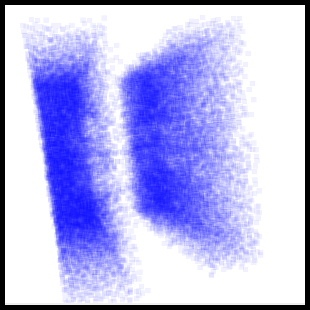
\includegraphics[width=50mm]{waterpoint}
  \end{center}
  \caption{Water point visualisation. Each point represents a water molecule.}
  \label{fig:implementation_waterpoint}
\end{figure}

% }}}

\subsection{Balls and stick}
% {{{
\label{sub:implementation_ballstick}

% TODO: more info, how chosen, how selected

For the ball and stick visualisation technique, the oxygen and hydrogen atoms
are represented by spheres. The spheres are rendered using different colours,
and at different sizes. The size and colour of the sphere can be changed by the
user. Lighting can be enabled to better see the spheres. See figure
\ref{fig:implementation_ballstick} where some water molecules are visible.

The red spheres represents the oxygen atoms, while the blue spheres represents
the hydrogen atoms. The left image uses the classical approach, where
cylinders are used to connect the atoms together. The right image uses the CPK
approach, where the atoms are enlarged to encompass the molecular bond.

% TODO: discuss
\begin{figure}[h!]
  \begin{center}
    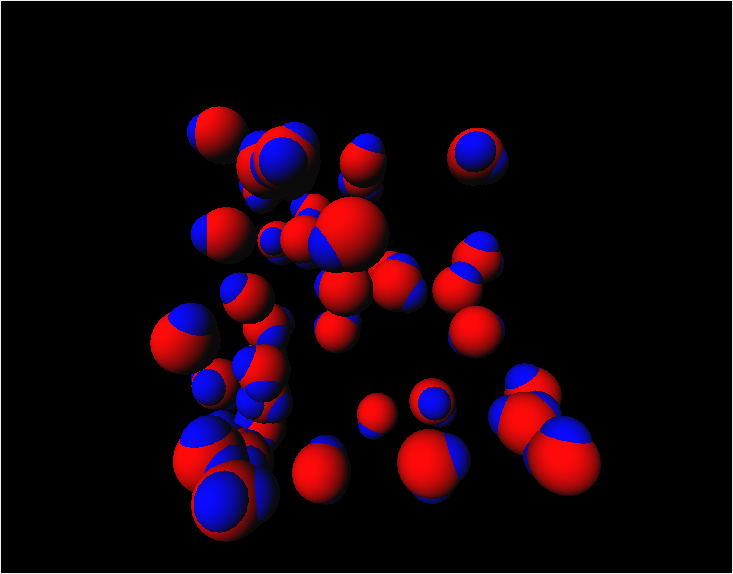
\includegraphics[width=100mm]{ballstick}
  \end{center}
  \caption{Ball and stick visualisation. The left image uses the classical
  approach, while the right image uses the CPK approach.}
  \label{fig:implementation_ballstick}
\end{figure}

% }}}

\subsection{Metaballs}
% {{{
\label{sub:implementation_metaballs}

% TODO: add to results section!!!
For the metaballs visualisation technique, the isosurface is extracted using
the marching cubes algorithm. Both the marching cubes and marching tetrahedron
algorithms were implemented and tested. The marching cubes algorithm is used
and not marching tetrahedrons as it produced fewer triangles. Otherwise, the
surface quality and computational cost of marching cubes and marching
tetrahedrons are comparable and thus the algorithm that produces fewer
triangles is preferred (marching cubes).

As was mentioned in Section \ref{sec:implementation_details}, the GTS library
is used to perform the surface decimation. Due to unforeseen difficulties and
time constraints, using a library was the fastest way to achieve decimation.

The computational cost for a single frame for the metaballs visualisation
technique is quite high. A frame can be generated in real time for small
volumes only (less than 500 water molecules). Larger volumes may take upwards
of 5 seconds or more for a single frame to be generated. Performing decimation
on the extracted surface will only make the time delay worse. See Chapter
\ref{cha:results} for results and an analysis on the computation costs of the
surface extraction and decimation.

A pre-processing option is available for the metaballs visualisation technique.
All the frames can be pre-processed and saved to file. The output file is a
simple dump of the vertices and normals of all the triangles. This file can
then be used to render the surface without the processing overhead.

When rendering the surface, one side of the surface is coloured blue, while the
other is coloured green. This allows differentiation of the sides of the
surface. The blue side of the surface is facing the non-water area of the
volume, while the green side of the surface is facing towards the water area.
The volume used for Figure \ref{fig:implementation_metaballs} is the same as
that used for Figure \ref{fig:implementation_waterpoint}. Figure
\ref{fig:implementation_metaballs} clearly shows the boundary between the water
and non-water parts of the volume.

To help see the surface detail, lighting can be enabled.

% TODO: discuss
\begin{figure}[h!]
  \begin{center}
    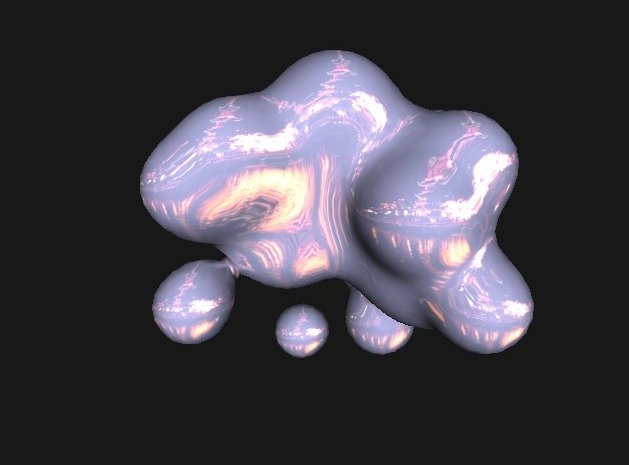
\includegraphics[width=50mm]{metaballs}
  \end{center}
  \caption{Metaballs visualisation, where the surface is easily visible.}
  \label{fig:implementation_metaballs}
\end{figure}

% }}}

\subsection{Water cluster}
% {{{
\label{sub:implementation_cluster}

The water molecules in the water clusters are joined by cylinders, spheres are
then drawn at the end points. Lighting can be enabled for this visualisation
technique so that the shape and orientation of the cylinders can be more easily
determined. See figure \ref{fig:implementation_watercluster} for an image
showing a few water clusters.

% TODO: discuss
\begin{figure}[h!]
  \begin{center}
    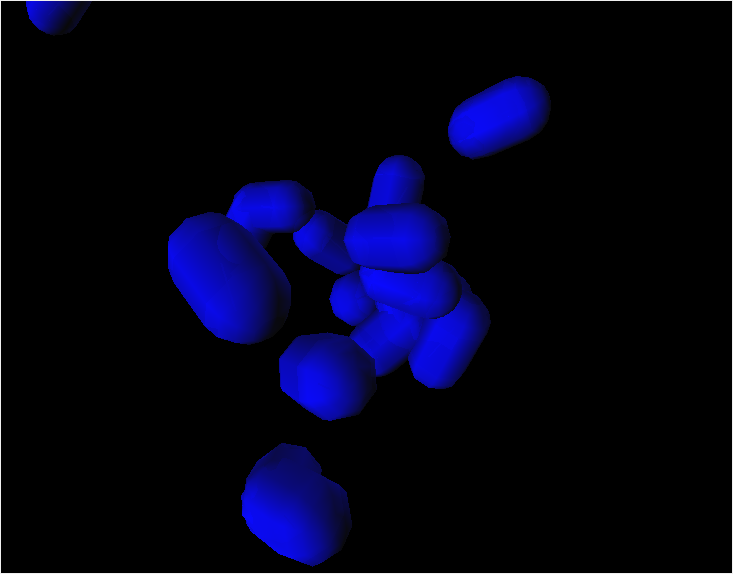
\includegraphics[width=50mm]{watercluster}
  \end{center}
  \caption{Water cluster visualisation, each water cluster is visible.}
  \label{fig:implementation_watercluster}
\end{figure}

% }}}

\subsection{Quantisation error}
% {{{
\label{sub:implementation_quantisation}

The distance between the unquantised and quantised positions of the water
molecules represents the error introduced by quantisation. Visualising the error is
accomplished by either rendering a point for the water molecule, or a line
between unquantised and quantised positions. The colour of the point/line is
linked to the magnitude of the error on a standard cold-hot colour scale [REF].
% TODO: cite cold-hot colour scale

As the errors are uniformly distributed, having the colour linearly
proportional to the error value produces poor results: the large error values
do not stand out clearly. Instead, the colour scale is stepped so that the
large error values are clearly visible.

The colour scale is determined using two error thresholds. If the error value
is less than the lower threshold, then the error is ignored and nothing is
rendered. If the error value is between the two threshold values, then the
colour is determined linearly up until the midpoint value, where the colour is
set to the final error colour. See figure \ref{fig:implementation_quantgraph}
for a graph illustrating how the colour is determined.

Figure \ref{fig:implementation_quanterror} shows the quantisation errors for an
example volume.

% TODO: discuss, add labels, interpolate colours, colour range
\begin{figure}[h!]
  \begin{center}
    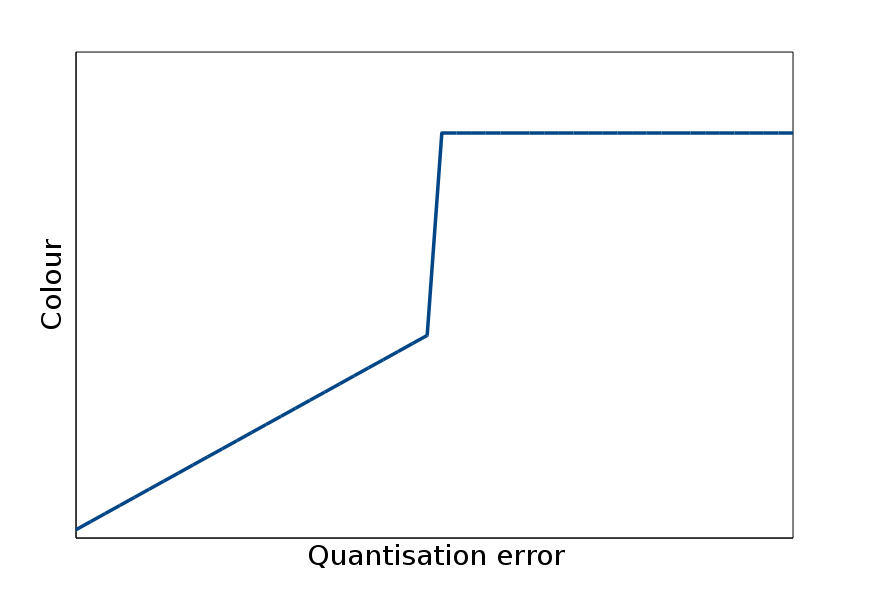
\includegraphics[width=80mm]{quant_colour_graph}
  \end{center}
  \caption{Graph illustrating stepped colour assignment for quantisation error.}
  \label{fig:implementation_quantgraph}
\end{figure}

% TODO: discuss
\begin{figure}[h!]
  \begin{center}
    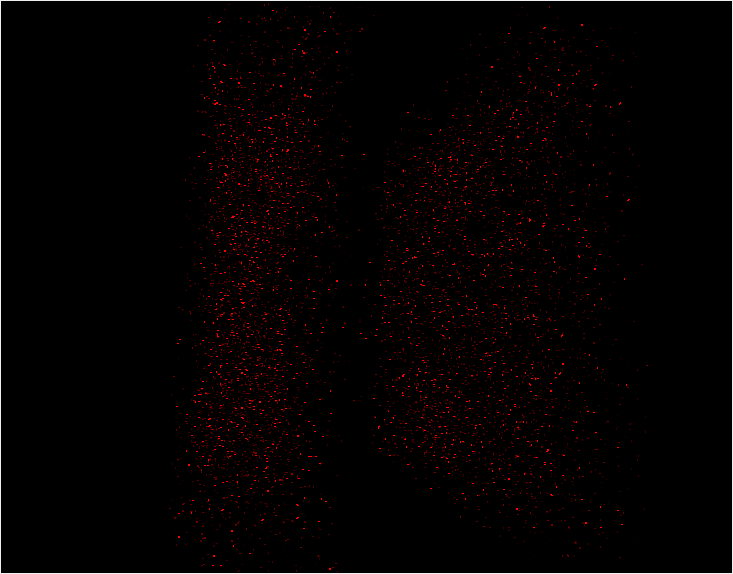
\includegraphics[width=50mm]{quanterror}
  \end{center}
  \caption{Quantisation error visualisation, highlights large quantisation
  errors.}
  \label{fig:implementation_quanterror}
\end{figure}

% }}}

% }}}

\section{Limitations}
% {{{
\label{sec:implementation_limitations}

As the data can be very different, some adjustments to various configuration
values will need to be made to most effectively visualise the data. An example
of such a change is the alpha value and point size for the water point
visualisation technique. For small volumes, a higher alpha value and point size
will be needed to effectively visualise the volume. Other changes need to be
made for all the other visualisation techniques. These changes are
unfortunately unavoidable.

The water point visualisation technique is only useful for volumes where there
are large amounts of water, and there is also a large area where there is no
water. If the volume is small or uniformly filled with water molecules, the
alpha effects will not be significant.

The metaballs visualisation technique requires considerable processing for each
frame (surface extraction and decimation), hence real time rendering is only
possible for small volumes. The amount of rendering time required is dependant
on the number of water molecules and extracted surface, processing time for a
single frame can be from a few seconds, up to a minute. Disabling decimation
will decrease the time required for a single frame, processing time then ranges
from a few hundred milliseconds, up to 10 seconds.

There is an option to pre-process the volume and save the extracted surfaces to
file, however, the generated files are generally considerably larger than the
DCD file. The size of the pre-processed file is dependant on the number of
water molecules and number of frames. From the data used for the quantisation
experiment, the pre-processed file was an average of 10 times larger than the
DCD file. The smallest output file was the same size as the DCD file, while the
largest was 100 times larger.

To limit the file size and pre-processing time, the number of frames to
pre-process is limited. This number can be set by the user.

% }}}

% }}}

